\section{Recadrage de l'image}
\begin{enumerate}
  \item \q{Ecrire une fonction qui retourne une image couleur qui a pour
          dimension la moitié de l’image initiale et qui place le véhicule au
          centre si l’excentration le permet. Sinon, on montrera l’image au
          mieux.}

  \item \q{Faire afficher cette image.}

        \codeFromFileT{helpers/image.py}{section-06/q1-1.py}
        \codeFromFileT{main.py}{section-06/q1-2.py}
        Sans aucun recadrage cette fois-ci :
        \begin{center}
          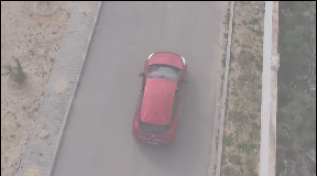
\includegraphics[scale=0.8]{section-06/q1-3.png}
        \end{center}
\end{enumerate}
